\documentclass[11pt,a4paper]{article}
\usepackage{amsmath,amssymb,amsthm}
\usepackage{algorithm,algorithmic}
\usepackage{graphicx}
\usepackage{tikz}
\usetikzlibrary{bayesnet,arrows.meta,positioning}
\usepackage{hyperref}
\usepackage{cleveref}

% Theorem environments
\newtheorem{definition}{Definition}
\newtheorem{theorem}{Theorem}
\newtheorem{lemma}{Lemma}
\newtheorem{proposition}{Proposition}
\newtheorem{corollary}{Corollary}
\newtheorem{remark}{Remark}

% Custom commands
\DeclareMathOperator{\Cat}{Cat}
\DeclareMathOperator{\Ber}{Ber}
\DeclareMathOperator{\supp}{supp}
\newcommand{\E}{\mathbb{E}}
\newcommand{\Prob}{\mathbb{P}}
\newcommand{\cA}{\mathcal{A}}
\newcommand{\cS}{\mathcal{S}}
\newcommand{\cT}{\mathcal{T}}
\newcommand{\cN}{\mathcal{N}}
\newcommand{\cP}{\mathcal{P}}
\newcommand{\cE}{\mathcal{E}}

\title{The AlphaZX Distribution: A Hierarchical Mixed Discrete Distribution for Structured Action Spaces in Graph Rewriting}
\author{A Technical Note on Elegant Compositional Design}
\date{\today}

\begin{document}

\maketitle

\begin{abstract}
We present the AlphaZX Distribution, a novel hierarchical probability distribution designed for sampling complex, structured actions in graph rewriting systems. This distribution elegantly factorizes an exponentially large discrete action space into a sequence of conditional distributions, each capturing a different aspect of the graph transformation. The design demonstrates how careful probabilistic modeling can make intractable combinatorial spaces computationally feasible while maintaining exact likelihood computation and efficient sampling. We provide a formal mathematical characterization, analyze its theoretical properties, and discuss its connections to existing frameworks in probabilistic graphical models and reinforcement learning.
\end{abstract}

\section{Introduction}

Consider the challenge of defining a probability distribution over actions that transform quantum circuit graphs. Each action consists of selecting:
\begin{itemize}
    \item A rewrite rule type from a discrete set
    \item A specific node in the graph where the rule applies
    \item A phase parameter for quantum operations
    \item A set of new edges to add
    \item A subset of existing edges to transfer
\end{itemize}

The naive approach would require a categorical distribution over the product space of all these choices, resulting in a distribution with potentially billions of categories. The AlphaZX Distribution solves this through an elegant hierarchical factorization that respects the natural dependencies in the action structure.

\section{Mathematical Formulation}

\subsection{Action Space Structure}

Let us formally define the structured action space. An action $a \in \cA$ is a tuple:
\[
a = (t, n, \phi, e_{\text{new}}, e_{\text{transfer}})
\]
where:
\begin{itemize}
    \item $t \in \cT = \{1, 2, \ldots, |\cT|\}$ is the rewrite type
    \item $n \in \cN(t, s) \subseteq V(G)$ is a node from the graph $G$ valid for type $t$ in state $s$
    \item $\phi \in \cP$ is a phase from a discrete set of quantum phases
    \item $e_{\text{new}} \in \{0, 1, \ldots, k_{\text{max}}\}$ is the number of new edges
    \item $e_{\text{transfer}} \in \{0,1\}^{|E_{\text{eligible}}(n)|}$ indicates which edges to transfer
\end{itemize}

\subsection{Hierarchical Factorization}

The AlphaZX Distribution defines a probability measure over $\cA$ through the following factorization:

\begin{definition}[AlphaZX Distribution]
Given state $s \in \cS$, the AlphaZX Distribution $\pi(\cdot|s)$ over actions is defined as:
\begin{align}
\pi(a|s) &= \pi(t, n, \phi, e_{\text{new}}, e_{\text{transfer}}|s) \\
&= \pi_{\text{type}}(t|s) \cdot \pi_{\text{node}}(n|t,s) \cdot \pi_{\text{phase}}(\phi|t,n,s) \\
&\quad \cdot \pi_{\text{new}}(e_{\text{new}}|t,n,s) \cdot \pi_{\text{transfer}}(e_{\text{transfer}}|t,n,s)
\end{align}
\end{definition}

This factorization induces a directed graphical model:

\begin{center}
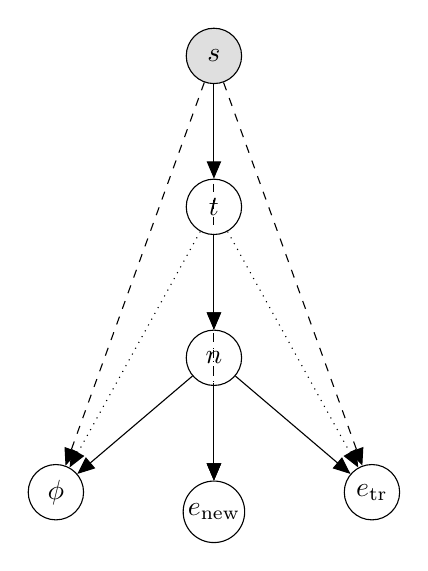
\begin{tikzpicture}
  % Define nodes
  \node[obs] (s) {$s$};%
  \node[latent, below=1.2 of s] (t) {$t$};%
  \node[latent, below=1.2 of t] (n) {$n$};%
  \node[latent, below left=1.2 and 1.5 of n] (phi) {$\phi$};%
  \node[latent, below=1.2 of n] (new) {$e_{\text{new}}$};%
  \node[latent, below right=1.2 and 1.5 of n] (trans) {$e_{\text{tr}}$};%

  % Define edges - tikz-bayesnet automatically styles them
  \edge{s}{t}
  \edge{t}{n}
  \edge{n}{phi,new,trans}

  % Additional edges from s (state conditions on everything)
  \edge[dashed]{s}{n,phi,new,trans}

  % Additional edges from t
  \edge[dotted]{t}{phi,new,trans}
\end{tikzpicture}
\end{center}

The hierarchical structure is perhaps more clearly shown as a flow diagram:

\begin{center}
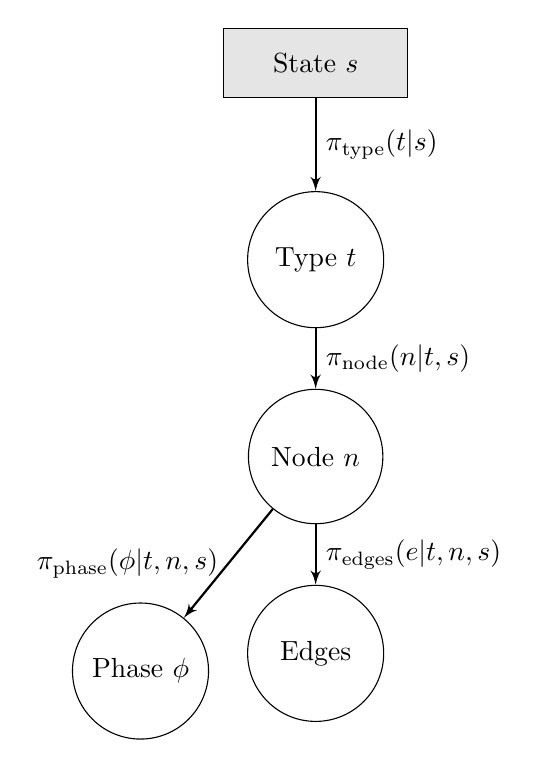
\begin{tikzpicture}[node distance=2.5cm, auto]
  % Define styles
  \tikzstyle{block} = [rectangle, draw, text width=6em, text centered, minimum height=2.5em]
  \tikzstyle{decision} = [circle, draw, text width=4em, text centered, minimum height=2.5em]
  \tikzstyle{line} = [draw, -latex', thick]

  % Place nodes
  \node [block, fill=gray!20] (state) {State $s$};
  \node [decision, below of=state] (type) {Type $t$};
  \node [decision, below of=type] (node) {Node $n$};
  \node [decision, below left=1.5cm and 1cm of node] (phase) {Phase $\phi$};
  \node [decision, below of=node] (edges) {Edges};

  % Draw edges with labels
  \path [line] (state) -- node {$\pi_{\text{type}}(t|s)$} (type);
  \path [line] (type) -- node {$\pi_{\text{node}}(n|t,s)$} (node);
  \path [line] (node) -- node[left] {$\pi_{\text{phase}}(\phi|t,n,s)$} (phase);
  \path [line] (node) -- node[right] {$\pi_{\text{edges}}(e|t,n,s)$} (edges);
\end{tikzpicture}
\end{center}

\subsection{Component Distributions}

Each component in the factorization has a specific parametric form that depends on the rewrite type:

\begin{enumerate}
    \item \textbf{Type Selection}: $\pi_{\text{type}}(t|s) = \Cat(t; \theta_{\text{type}}(s))$

    where $\theta_{\text{type}}(s) \in \Delta^{|\cT|-1}$ is computed by a neural network.

    \item \textbf{Node Selection}: $\pi_{\text{node}}(n|t,s) = \Cat(n; \theta_{\text{node}}(t,s))$

    The support depends on $t$: only nodes of the appropriate type for rewrite rule $t$ have non-zero probability.

    \item \textbf{Phase Selection}:
    \[
    \pi_{\text{phase}}(\phi|t,n,s) = \begin{cases}
    \Cat(\phi; \theta_{\text{phase}}(t,n,s)) & \text{if } t \in \cT_{\text{phase}} \\
    \delta_0(\phi) & \text{otherwise}
    \end{cases}
    \]

    where $\cT_{\text{phase}} \subseteq \cT$ is the set of rewrite types requiring phase selection (e.g., spider fission), and $\delta_0$ is the Dirac delta at $\phi = 0$.

    \item \textbf{New Edge Count}:
    \[
    \pi_{\text{new}}(e_{\text{new}}|t,n,s) = \begin{cases}
    \Cat(e_{\text{new}}; \theta_{\text{new}}(t,n,s)) & \text{if } t \in \cT_{\text{edges}} \\
    \delta_0(e_{\text{new}}) & \text{otherwise}
    \end{cases}
    \]

    \item \textbf{Edge Transfer}:
    \[
    \pi_{\text{transfer}}(e_{\text{transfer}}|t,n,s) = \begin{cases}
    \prod_{i} \Ber(e_{\text{transfer},i}; \theta_{\text{transfer},i}(t,n,s)) & \text{if } t \in \cT_{\text{edges}} \\
    \delta_{\emptyset}(e_{\text{transfer}}) & \text{otherwise}
    \end{cases}
    \]

    where $\delta_{\emptyset}$ assigns probability 1 to the empty set of transferred edges.
\end{enumerate}

\begin{remark}[On Conditional Structure]
The use of point mass distributions (Dirac deltas) for unused components is crucial for maintaining a valid probability distribution. When a rewrite type doesn't require certain components, those variables take deterministic default values with probability 1, ensuring the full joint distribution remains normalized. This design elegantly handles the variable structure of different rewrite operations.
\end{remark}

\section{Theoretical Properties}

\subsection{Consistency and Coherence}

\begin{theorem}[Consistency]
The AlphaZX Distribution defines a valid probability measure over $\cA$. That is:
\[
\sum_{a \in \cA} \pi(a|s) = 1 \quad \forall s \in \cS
\]
\end{theorem}

\begin{proof}
By the chain rule of probability and the fact that each component distribution is normalized (including the point mass distributions):
\begin{align}
\sum_{a \in \cA} \pi(a|s) &= \sum_t \pi_{\text{type}}(t|s) \sum_{n \in \cN(t,s)} \pi_{\text{node}}(n|t,s) \\
&\quad \times \sum_\phi \pi_{\text{phase}}(\phi|t,n,s) \sum_{e_{\text{new}}} \pi_{\text{new}}(e_{\text{new}}|t,n,s) \\
&\quad \times \sum_{e_{\text{transfer}}} \pi_{\text{transfer}}(e_{\text{transfer}}|t,n,s)
\end{align}

For each $t$, the inner sums equal 1 because:
- If $t \in \cT_{\text{phase}}$: $\sum_\phi \Cat(\phi; \theta) = 1$
- If $t \notin \cT_{\text{phase}}$: $\sum_\phi \delta_0(\phi) = 1$ (all mass at $\phi = 0$)

Similarly for the edge components. Therefore:
\[
\sum_{a \in \cA} \pi(a|s) = \sum_t \pi_{\text{type}}(t|s) \cdot 1 \cdot 1 \cdot 1 \cdot 1 = 1
\]
\end{proof}

\subsection{Computational Complexity}

\begin{proposition}[Sampling Complexity]
Sampling from the AlphaZX Distribution requires $O(k + |E_{\text{eligible}}|)$ operations, where $k$ is the number of components and $|E_{\text{eligible}}|$ is the number of eligible edges for transfer.
\end{proposition}

\begin{proposition}[Likelihood Complexity]
Computing $\log \pi(a|s)$ requires $O(k + |E_{\text{eligible}}|)$ operations.
\end{proposition}

Compare this to the naive categorical distribution over $\cA$, which would require $O(|\cA|)$ operations where $|\cA|$ can be exponentially large.

\subsection{Entropy and Information Theory}

The entropy of the AlphaZX Distribution admits a natural decomposition:

\begin{theorem}[Entropy Decomposition]
The entropy of the AlphaZX Distribution can be bounded as:
\begin{align}
H[\pi(\cdot|s)] &\leq H[\pi_{\text{type}}(\cdot|s)] + \E_{t \sim \pi_{\text{type}}}[H[\pi_{\text{node}}(\cdot|t,s)]] \\
&\quad + \E_{t,n}[H[\pi_{\text{phase}}(\cdot|t,n,s)]] + \E_{t,n}[H[\pi_{\text{new}}(\cdot|t,n,s)]] \\
&\quad + \E_{t,n}[H[\pi_{\text{transfer}}(\cdot|t,n,s)]]
\end{align}
\end{theorem}

This decomposition provides insights into which components contribute most to the exploration behavior in reinforcement learning applications.

\section{Elegance Through Design}

The AlphaZX Distribution exhibits several elegant design principles:

\subsection{Structural Coherence}
The factorization mirrors the logical structure of graph rewriting operations. First select what to do (type), then where to do it (node), then how to do it (phase, edges).

\subsection{Handling Operation-Specific Parameters}
Different graph rewrite operations require different parameters:
\begin{itemize}
    \item \textbf{Spider fusion}: Only requires selecting two adjacent nodes
    \item \textbf{Spider fission}: Requires a phase parameter and edge redistribution
    \item \textbf{Identity removal}: Only requires selecting an identity node
    \item \textbf{Bialgebra operations}: May require edge transfers but no phase
\end{itemize}

The distribution elegantly handles this heterogeneity through conditional point masses. When an operation doesn't require a parameter, that component collapses to a deterministic value, contributing a factor of 1 to the joint probability. This avoids the need for separate distribution classes for each operation type while maintaining mathematical coherence.

\subsection{Conditional Independence}
The distribution exploits conditional independence to reduce parameter count. For example, the phase selection doesn't need to consider all possible node-type combinations, only the specific $(t,n)$ pair sampled.

\subsection{Variable Support}
The support of each conditional distribution adapts to previous choices. This is handled elegantly through masking in the softmax computation.

Let $f_{\text{node}}: V(G) \times \cS \to \mathbb{R}$ be the neural network that computes logits for each node given the state. The node selection distribution is then:
\[
\pi_{\text{node}}(n|t,s) = \frac{\exp(f_{\text{node}}(n,s)) \cdot \mathbb{1}[n \in \cN(t,s)]}{\sum_{n' \in V(G)} \exp(f_{\text{node}}(n',s)) \cdot \mathbb{1}[n' \in \cN(t,s)]}
\]

where $\mathbb{1}[\cdot]$ is the indicator function. This can be implemented efficiently by setting logits of invalid nodes to $-\infty$ before applying softmax:

\[
\tilde{f}_{\text{node}}(n,s,t) = \begin{cases}
f_{\text{node}}(n,s) & \text{if } n \in \cN(t,s) \\
-\infty & \text{otherwise}
\end{cases}
\]

Then $\pi_{\text{node}}(n|t,s) = \text{softmax}(\tilde{f}_{\text{node}}(\cdot,s,t))_n$. This ensures only valid nodes for the selected rewrite type receive non-zero probability.

\subsection{Differentiability}
Despite the discrete nature and variable support, all operations remain differentiable with respect to the neural network parameters, enabling gradient-based learning.

\section{Implementation Insights}

The implementation leverages several sophisticated techniques:

\begin{algorithm}
\caption{Sampling from AlphaZX Distribution}
\begin{algorithmic}[1]
\STATE \textbf{Input:} State $s$, neural network parameters $\theta$
\STATE $t \sim \Cat(\theta_{\text{type}}(s))$
\STATE $\text{valid\_nodes} \gets \{n \in V(G) : n \in \cN(t,s)\}$
\STATE $n \sim \Cat(\theta_{\text{node}}(t,s)|_{\text{valid\_nodes}})$
\IF{$t$ requires phase}
    \STATE $\phi \sim \Cat(\theta_{\text{phase}}(t,n,s))$
\ELSE
    \STATE $\phi \gets 0$
\ENDIF
\STATE $e_{\text{new}} \sim \Cat(\theta_{\text{new}}(t,n,s))$
\STATE $e_{\text{transfer}} \sim \prod_i \Ber(\theta_{\text{transfer},i}(t,n,s))$
\STATE \textbf{Return} $(t, n, \phi, e_{\text{new}}, e_{\text{transfer}})$
\end{algorithmic}
\end{algorithm}

\section{Connections to Existing Frameworks}

\subsection{Probabilistic Graphical Models}
The AlphaZX Distribution implements a Bayesian network with a specific topology optimized for the action space structure. It belongs to the class of \emph{context-specific independence} models.

\subsection{Hierarchical Reinforcement Learning}
Unlike traditional HRL which focuses on temporal abstraction, this distribution provides \emph{structural abstraction} over the action space, related to the MAXQ framework but applied to action selection rather than value decomposition.

\subsection{Structured Prediction}
The distribution solves a structured prediction problem where the output has combinatorial constraints. It's related to structured SVMs and CRFs but maintains exact inference through careful factorization.

\section{Theoretical Implications}

\begin{remark}[On Expressiveness]
Despite the factorization, the AlphaZX Distribution can represent any distribution over valid actions by appropriate parameterization of the neural networks. The factorization provides an inductive bias rather than a limitation.
\end{remark}

\begin{remark}[On Scalability]
The hierarchical structure enables scaling to graphs with thousands of nodes where a flat distribution would be computationally intractable.
\end{remark}

\section{Conclusion}

The AlphaZX Distribution demonstrates how thoughtful probabilistic modeling can elegantly solve complex problems in discrete action spaces. Its hierarchical structure, theoretical grounding, and computational efficiency make it a compelling example of principled design in machine learning.

The key insight is that by factorizing the action space according to its natural structure, we can transform an intractable problem into a sequence of simple, conditional decisions. This not only makes computation feasible but also provides better inductive bias for learning.

\section*{Acknowledgments}

This distribution was developed for the AlphaZX project, applying reinforcement learning to quantum circuit optimization through graph rewriting. The elegance emerges from respecting the mathematical structure of the problem domain.

\end{document}